\documentclass[a4paper,11pt]{ujreport}

%%【PostScript, JPEG, PNG等の画像の貼り込み】
%% 利用するパッケージを選んでコメントアウトしてください.
\usepackage{graphicx} % for 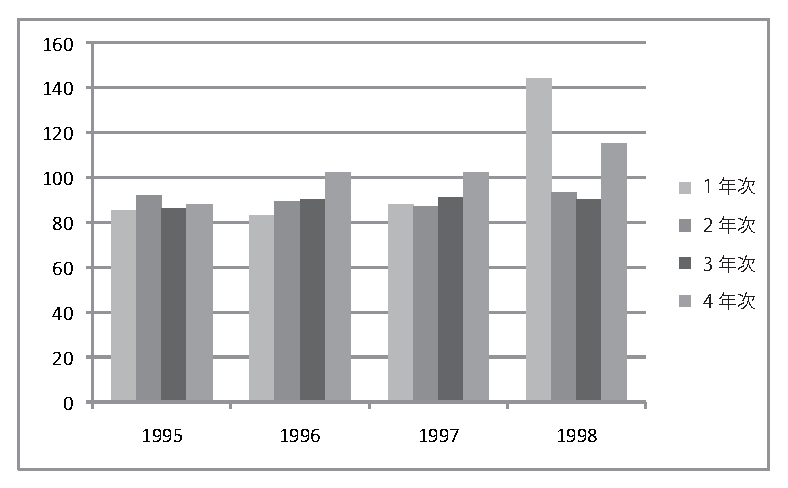
\includegraphics[width=3cm]{sample.eps}
\usepackage{epsfig} % for 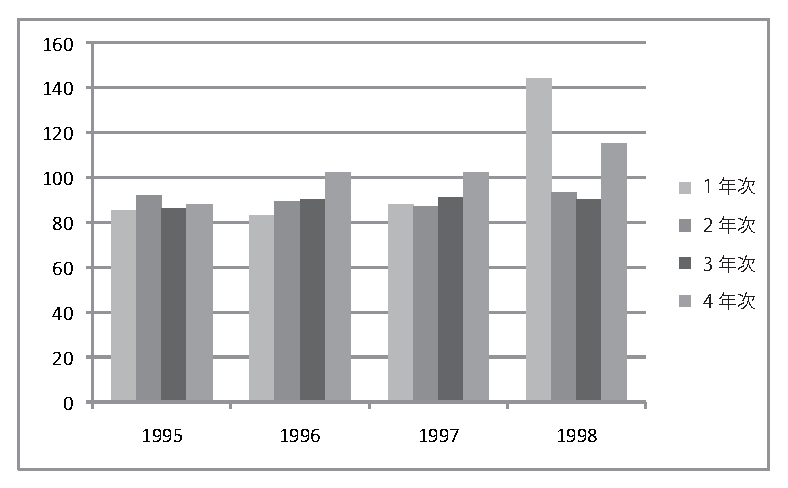
\psfig{file=sample.eps,width=3cm}
%\usepackage{epsf} % for \epsfile{file=sample.eps,scale=0.6}
%\usepackage{epsbox} % for \epsfile{file=sample.eps,scale=0.6}

\usepackage{times} % use Times Font instead of Computer Modern

\setcounter{tocdepth}{3}
\setcounter{page}{-1}

\setlength{\oddsidemargin}{0.1in}
\setlength{\evensidemargin}{0.1in}
\setlength{\topmargin}{0in}
\setlength{\textwidth}{6in}
%\setlength{\textheight}{10.1in}
\setlength{\parskip}{0em}
\setlength{\topsep}{0em}

%\newcommand{\zu}[1]{{\gt \bf 図\ref{#1}}}

%% タイトル生成用パッケージ(重要)
\usepackage{mast-jp-sjis}

%% タイトル
%% 【注意】タイトルの最後に\\ を入れるとエラーになります
\title{NoSQL型データベースシステムでの実体化ビュー選択に関する研究}
%% 著者
\author{高木 颯汰}
%% 指導教員
\advisor{古瀬 一隆 陳 漢雄}

%% 年月 (提出年月)
%% 年月は必要に応じて書き替えてください.
\majorfield{ } \yearandmonth{2019年 1月}



\begin{document}
\maketitle
\thispagestyle{empty}
\newpage

\thispagestyle{empty}
\vspace*{20pt plus 1fil}
\parindent=1zw
\noindent
%%
%% 論文の概要(Abstract)
%%
\begin{center}
	{\bf 概要}
	\vspace{5mm}
\end{center}
本論文ではNoSQLの一種であるドキュメント指向データベースに実体化ビューを導入する事によって問い合わせ処理を高速化する手法を提案する.ドキュメント指向データベースでは従来のリレーショナルデータベースにあったような参照型のデータ構造に加えて埋込型のデータ構造を選択できる.参照先の内容を埋め込む事によって結合処理をしなくて済むが,ファイルサイズが大きくなる傾向にあり,フラグメンテーションが発生し,逆にパフォーマンスが落ちる可能性がある.そこで本手法ではリレーショナルデータベースで実現されている実体化ビューの概念をNoSQLにも応用する事で,問い合わせ処理を自動的に高速化する.具体的には,頻繁に問い合わせのある結合処理や集計処理を自動的に検知してその部分のみ予め実体化することでデータベースアクセスの高速化を実現している.

%%%%%
\par
\vspace{0pt plus 1fil}
\newpage

\pagenumbering{roman} % I, II, III, IV
\tableofcontents
\listoffigures
%\listoftables

\pagebreak \setcounter{page}{1}
\pagenumbering{arabic} % 1,2,3


\chapter{はじめに}

数年前までは主要なデータストアとして,リレーショナルデータベースがあげられることがほとんどであった.それは多くの開発者がSQLに慣れ親しんでおり,正規化されたデータモデル,トランザクションの必要性,耐久性のあるストレージエンジンが提供する保証を受けられるからである\cite{Sky株式会社201212}.しかし近年高いスケーラビリティや大量なデータ処理が得意であることなどからNoSQLに対する需要が急激に増えている.

例えばNoSQLの一種のドキュメント指向データベースはデータベースの構造を表すスキーマを定義する必要がなく,大量なデータを事前準備なしで格納することができる.従来のリレーショナルデータベースにあったような参照型のデータ構造に加えて埋込型のデータ構造を選択できる.型宣言の必要のないスクリプト言語と相性が良いことなども合間って,プロトタイプを高速に開発することが求められるビジネスの現場で採用されることが増えている\cite{渡部201602}.

一方でドキュメント指向データベースの特徴とも言える階層的なデータモデルが更新処理速度の低下やデータ参照の柔軟性を低下を招くことがある.これを防ぐためにはドキュメントに階層的に埋め込むフィールドを適切に選択する必要がある.本論文ではこの選択の自動化し,ドキュメント指向データベースのデータモデルのチューニングを行い,データアクセスを高速化する.

本論文の構成は以下の通りである.まず,第2章において関連研究について紹介する.次に,第3章において本研究の提案手法について説明をし,第4章にて提案手法に関する実験を行う.第5章において実験の結果と考察を述べ,最後に第6章において本論文のまとめと今後の課題を示す.

\chapter{関連技術}
\section{Materialized View}
リレーショナルデータベースにおけるビュー (view) はリレーショナルデータモデルの発案者であるコッドにより導入された概念であり\cite{Codd1974RecentII},1つ以上の表(または他のビュー)から任意のデータを選択し,それらを表したものである.ビューの実体はデータを持たないSQL文であり,実行された際にはバックグラウンドでSELECT処理が毎回実行される.それに対して実体化ビュー(Materialized View)はビューと同じく複数の表の結合処理や集計処理を行うが,その結果を実際のテーブルに保持する.保持された実体化ビューは元のテーブルが更新されるたびに更新される.そのため,最新でない状態を取得する可能性はあるが,結合処理が必要ないため効率的なアクセスが可能になる.その一方,更新処理が増加するので実体化ビュー化する部分の選択は慎重に行う必要があり,この作業を自動化する研究が行われている\cite{mistry2001materialized}.図\ref{figure:MvDescription}は実体化ビューを図示したものである.
\begin{figure}[htbp]
	\begin{center}
		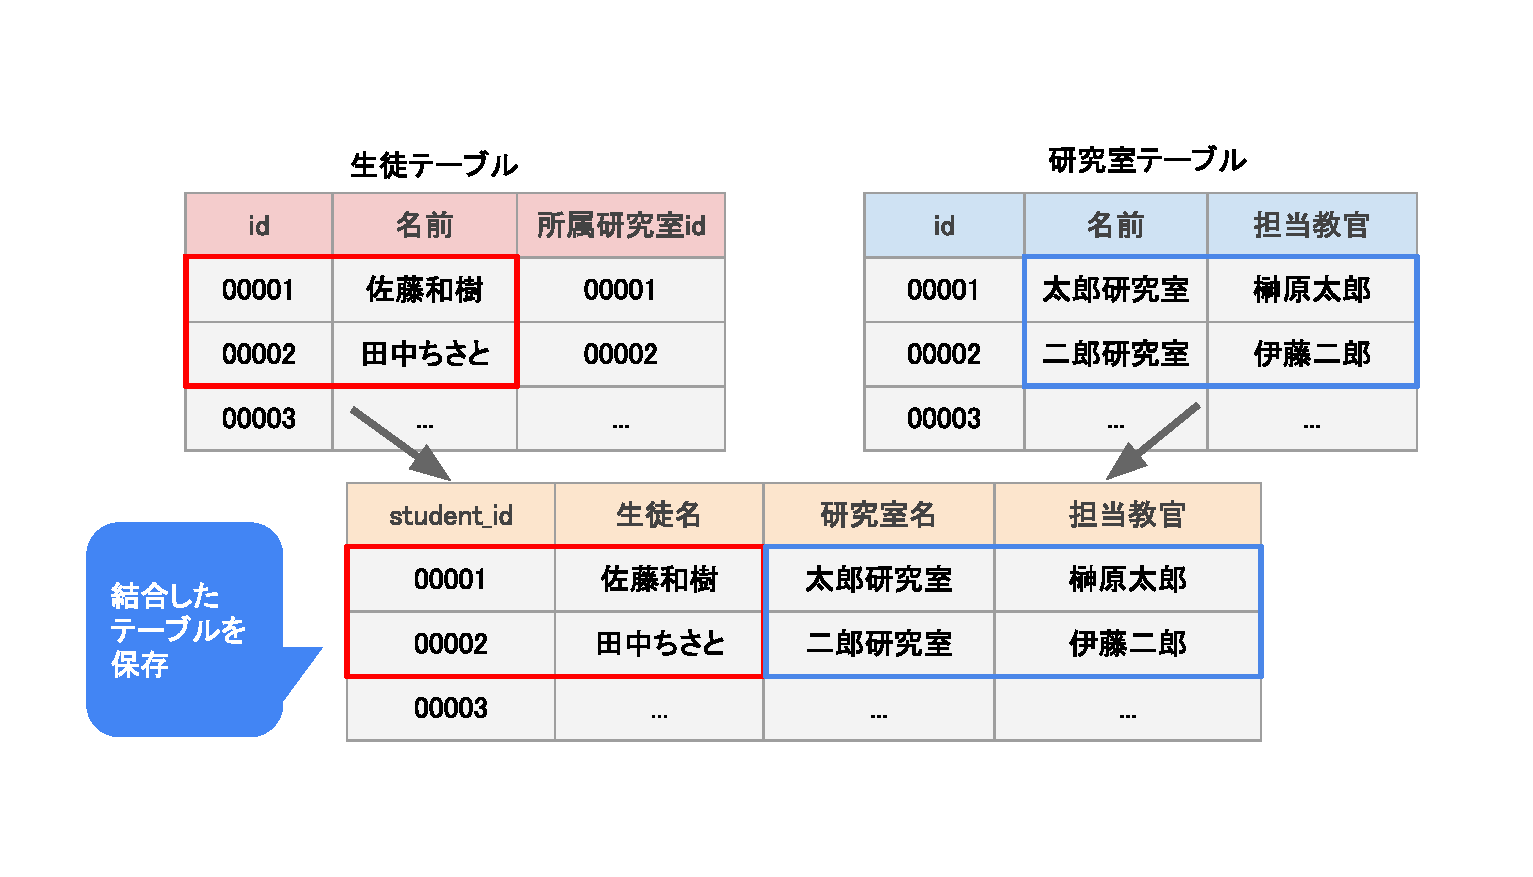
\includegraphics[width=30em, trim=0 5em 0 0]{src/MvDescription.eps} %[trim=left bottom right top]
	\end{center}
	\caption{実体化ビュー}
	\label{figure:MvDescription}
\end{figure}

\section{NoSQL}
NoSQLとは,“Not only SQL”の略称であり,SQLを用いないデータベースの総称を表す \cite{太田201204}.情報の大規模化が進み,ビッグデータと呼ばれる概念が登場すると共に,構造が複雑な様々なデータが登場するようになった.NoSQLは,そのような複雑な構造のデータに柔軟に対応し処理を行うことができる.GoogleやAmazon,Twitterなど,世界的規模を誇る企業がNoSQLデータベースを利用しており,今後ますますデータの大規模化が進む現代社会において,重要な役割を果たすデータベースである\cite{太田201204}.
NoSQLデータベースはキー・バリュー型,カラム指向型,ドキュメント指向型,グラフ型の4種類の型に大別することができる.キー・バリュー型は,インデックスであるキーと値であるバリューのペアでデータが構成され,キーを指定することでデータを呼び出すことができる.カラム指向型は行に対してキーが付され,それが複数の列(カラム)に対応する形のデータモデルである.ドキュメント指向型は,JSONやXMLなどの形式で記述されたドキュメントの形でデータを扱うデータモデルである.グラフ型は,データ間の関係性をグラフの構造で表すデータモデルである\cite{太田201204}.

\section{MongoDB}
MongoDBとは,JSONやXMLなどの形式で記述されたドキュメント指向型のデータを扱うNoSQLデータベースの代表的なものの一つである.RDBとは違い,スキーマの定義を必要としない\cite{太田201204}\cite{mongodb}.また,JSON形式のデータを扱うため,Webシステムなどに利用しやすい.
MongoDBにおいては,RDBのテーブルにあたるものとしてコレクション,RDBの行にあたるものとしてドキュメント,RDBの列にあたるものとしてフィールドというデータ構想が使われる.
ドキュメント指向型データベースの特徴として埋め込み(embed)がある.従来のRDBでは複数の表による1対多や多対多の関係を表す際に,参照先のプライマリーキーのみを保存してSELECTされる際に結合処理を行う.それに対してドキュメント指向型データベースでは参照先の実データを参照元に埋め込むことができ,これによって結合処理を省くことができる.埋め込み先が複数の場合には更新処理が増加し,従来の参照型に比べてデータアクセスの柔軟性が損なわれるというデメリットがある\cite{Sky株式会社201212}.図\ref{EmbedReference}はドキュメント指向型データベースの参照型を埋込型を表した図である.
\begin{figure}[htbp]
	\begin{center}
		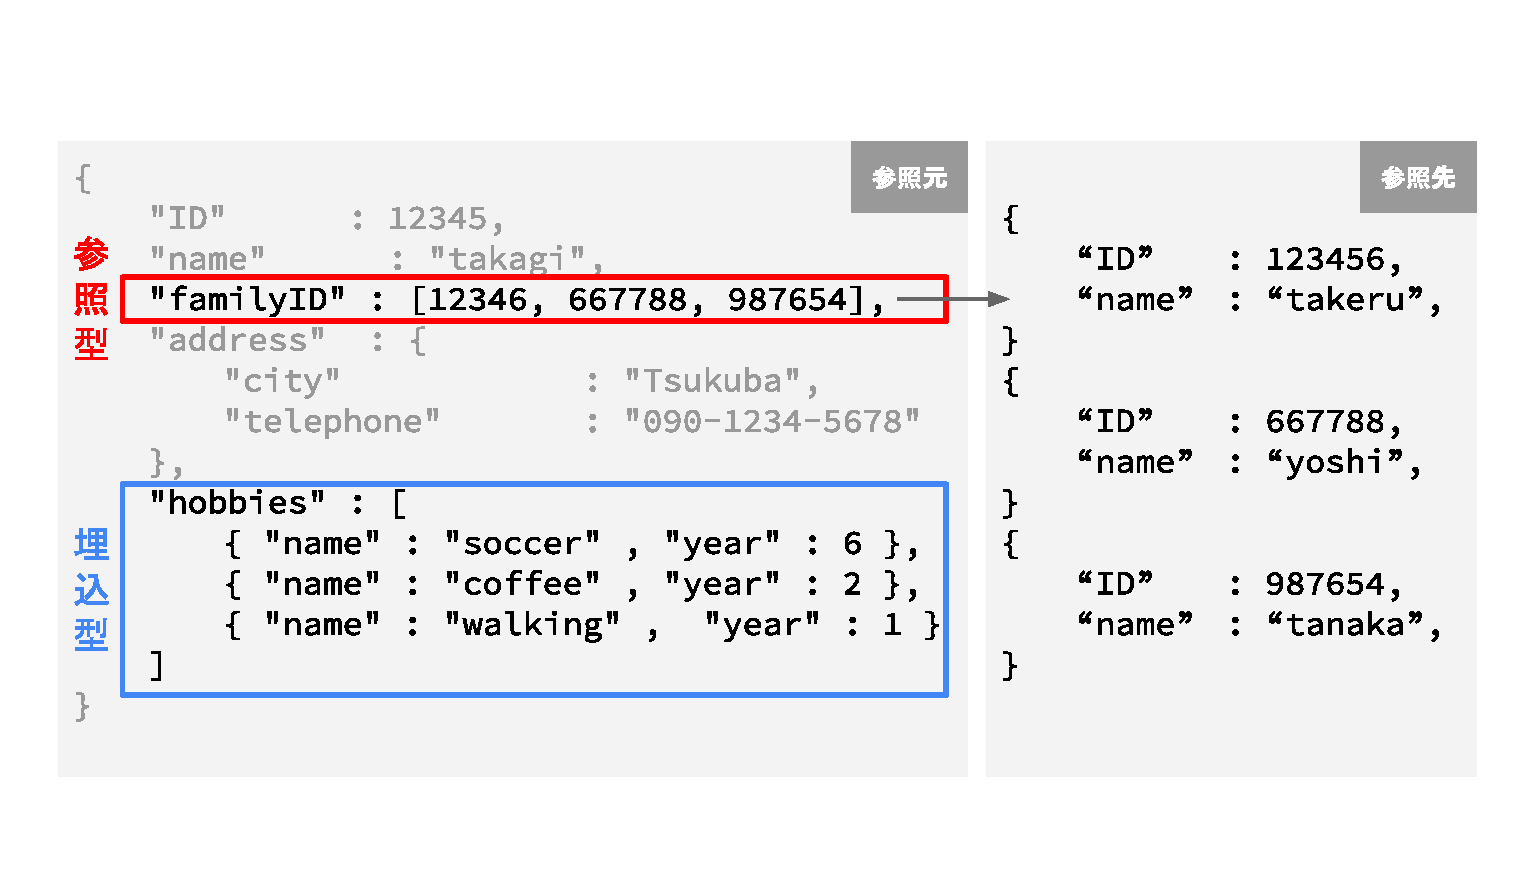
\includegraphics[width=30em, trim=0 5em 0 0]{src/EmbedReference.eps} %[trim=left bottom right top]
	\end{center}
	\caption{参照型と埋込型}
	\label{EmbedReference}
\end{figure}

\section{Restful API}
RESTとはRoy Fieldingが提唱した概念であり\cite{fielding2000architectural},“REpresentational State Transfer”の略である.分散システムにおける複数のソフトウェアを連携させるのに適した考え方であり,やりとりされる情報はそれ自体で完結して解釈できるステートレス性,全てのリソースが一意的なアドレスを持つアドレス可能性,他の基盤的な機能を用いずに別の情報や状態を含むことで他のリソースを参照できる持続性,HTTPメソッド(“GET”や“POST”など)の統一インターフェースを提供していることなどの原則から成る.RESTの原則に則り構築されたHTTPの呼び出しインターフェースをRESTful APIと呼ぶ.本論文ではRESTful APIをミドルウェアに実装し実験を行う.

\chapter{提案手法}
\section{実装システムについて}
本論文ではドキュメント指向型データベースの埋込型データモデルをリレーショナルデータベースの実体化ビューと置き換えて考える.ドキュメント指向型データベースのよくアクセスされる部分や処理速度がネックとなっている部分を埋込型として別コレクションに保持することで“実体化ビュー作成”,どの部分を埋込型にするかの判断を“実体化ビュー選択”とする.図\ref{ReferenceToEmbed}は本論文での“実体化ビュー作成”を示したものである.
\begin{figure}[htbp]
	\begin{center}
		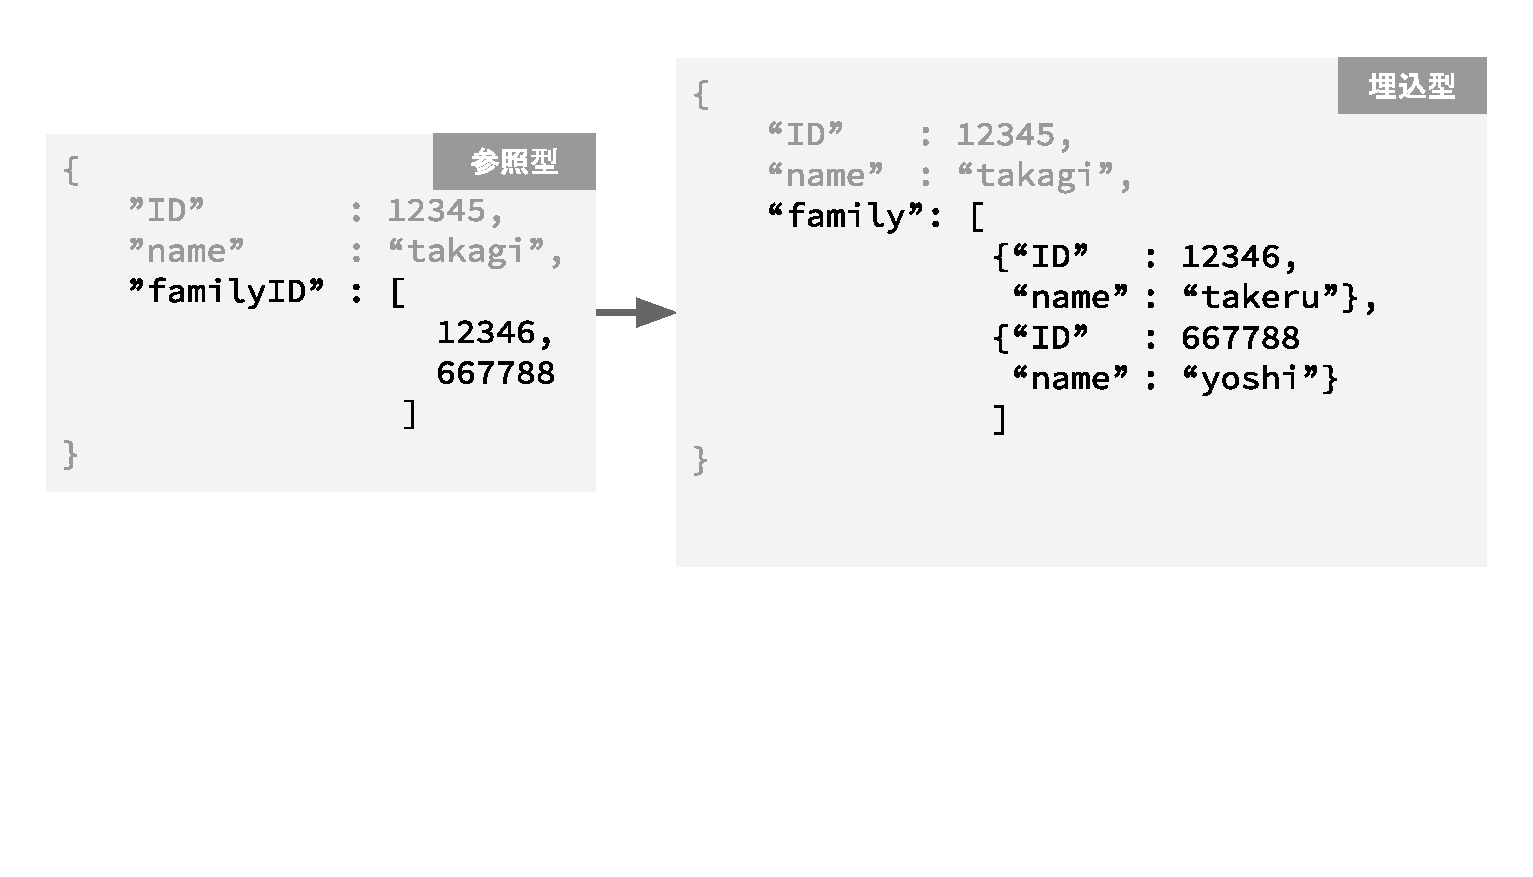
\includegraphics[width=30em, trim=0 13em 0 0]{src/ReferenceToEmbed.eps} %[trim=left bottom right top]
	\end{center}
	\caption{参照型から埋込型への書き換え}
	\label{ReferenceToEmbed}
\end{figure}

実装システムについて図\ref{Midleware}に示す.ユーザーからのデータアクセスから実体化ビュー作成までの流れを図\ref{Midleware}を用いて説明する.
\begin{figure}[h]
	\begin{center}
		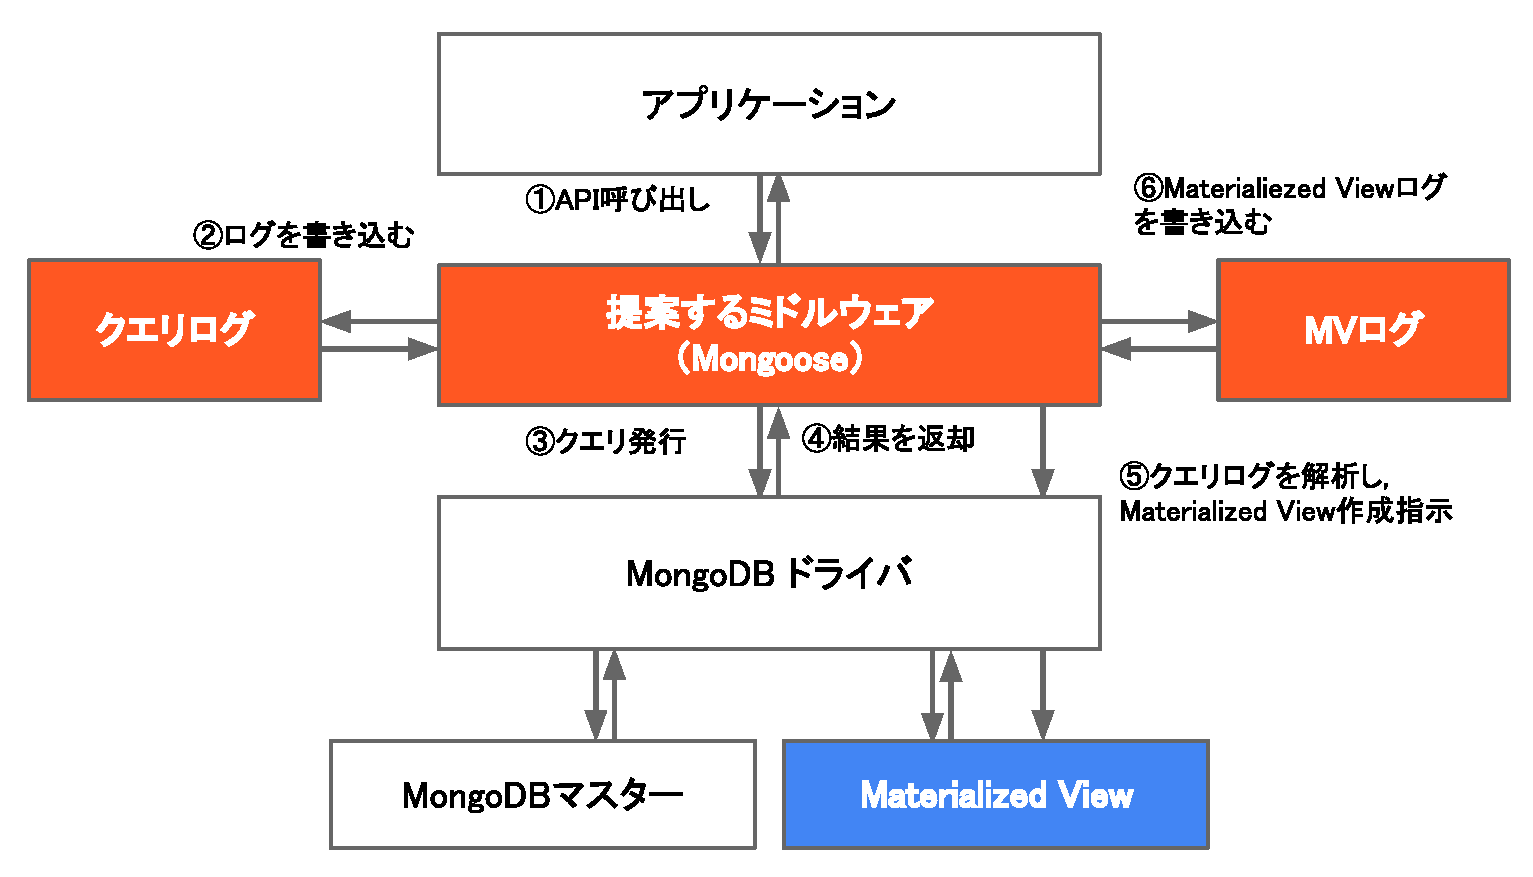
\includegraphics[width=30em]{src/Midleware.eps}
	\end{center}
	\caption{提案ミドルウェア(実体化前)}
	\label{Midleware}
\end{figure}
図\ref{Midleware}-①まずユーザーがアプリケーションからミドルウェアに対してデータアクセスの要求する.図\ref{Midleware}-②ミドルウェアでは,頻繁にアクセスされるドキュメントを分析するために,クエリに関するログを残す.図\ref{Midleware}-③次にMongoDBに対してクエリを発行する.図\ref{Midleware}-④MongoDBから返ってきたクエリセットをアプリケーションに返却する.図\ref{Midleware}-⑤クエリログを解析し,ボトルネックとなっているところや呼び出し回数の多い条件の実体化ビューを作成する.図\ref{Midleware}-⑥実体化したドキュメントに関してログに記録する.

実体化した後のデータアクセスの流れを図\ref{MidlewareMv}に示す.図\ref{MidlewareMv}-①’アプリケーションからデータベースにアクセスがあった場合,まずログからアクセスされたデータが実体化されているか判定する.図\ref{MidlewareMv}-②’実体化されている場合はクエリを書き換えて実体化ビューから結果を取得する.図\ref{MidlewareMv}-③’アプリケーションに結果を返す際には元のクエリに合うように適宜変換する.
\begin{figure}[htbp]
	\begin{center}
		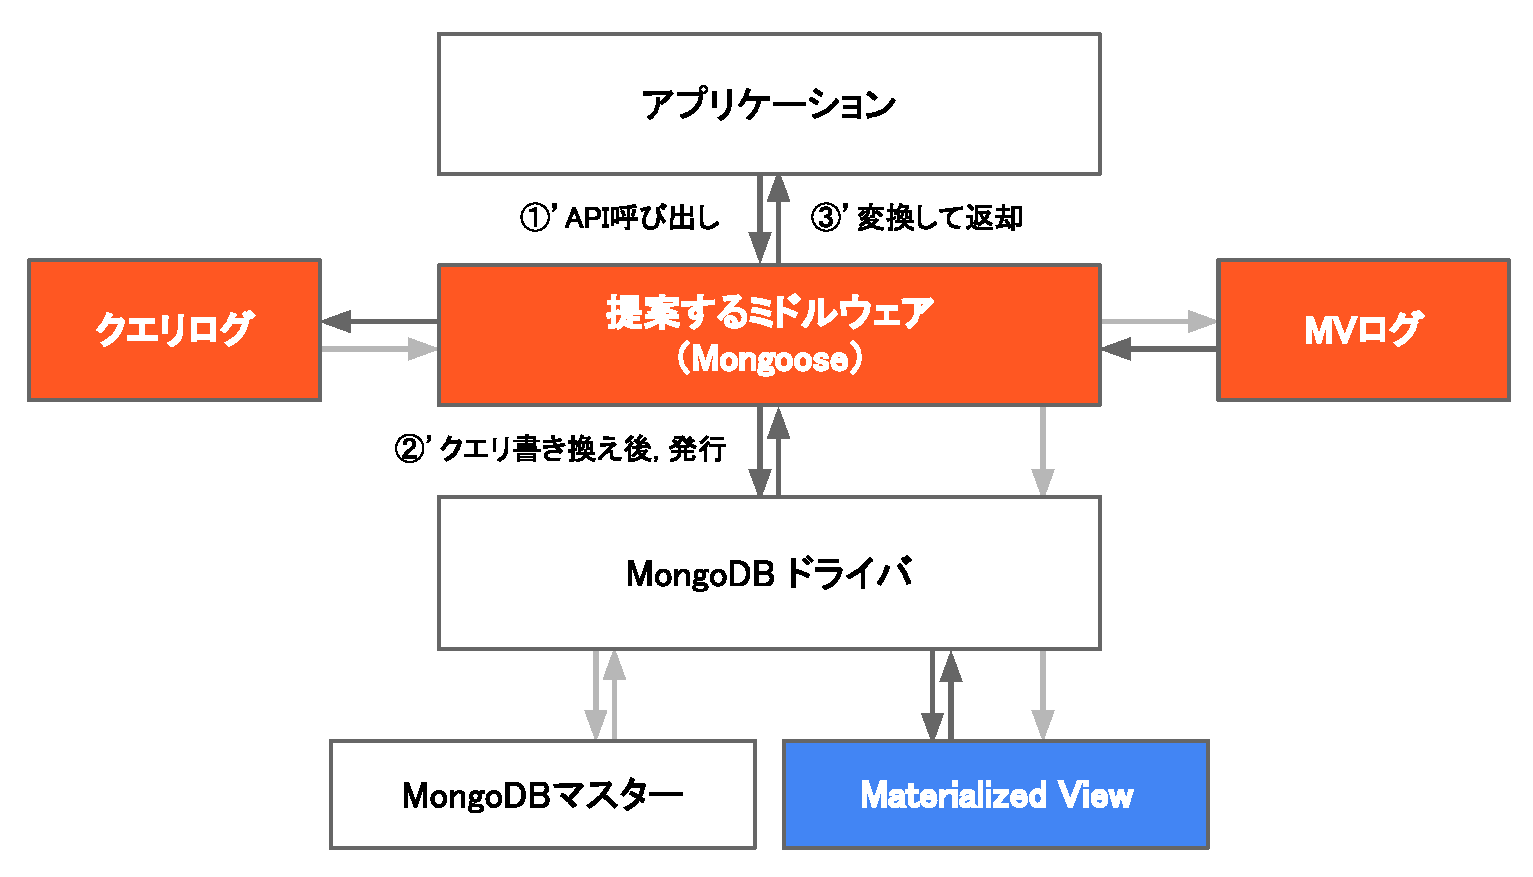
\includegraphics[width=30em]{src/MidlewareMv.eps} %[trim=left bottom right top]
	\end{center}
	\caption{提案ミドルウェア(実体化後)}
	\label{MidlewareMv}
\end{figure}


\chapter{実験}
\section{Mongooseについて}
MongooseとはMongoDB用モデリングツールで,Node.jsの非同期環境でうまく動作することを目的として設計されている.Mongooseを使用すれば,モデルを定義して操作することで,MongoDBのコレクション/ドキュメントを操作できる\cite{mongoose}.本論文ではMongooseを用いてMongoDBを操作するミドルウェアを実装する.





\chapter*{謝辞}
\addcontentsline{toc}{chapter}{\numberline{}謝辞}
本研究を進めるにあたり,指導教員の古瀬一隆先生と陳漢雄先生から,丁寧かつ熱心なご指導を賜りました.ここに感謝の意を表します.
また,研究室での議論を通じ,多くの知識をいただいたDSE研究室の皆様に感謝いたします.

\newpage

\addcontentsline{toc}{chapter}{\numberline{}参考文献}
\renewcommand{\bibname}{参考文献}

%% 参考文献
\bibliography{MaterializedView}
\bibliographystyle{junsrt}
%% [compile] upbibtex sample; uplatex sample; uplatex sample;


\end{document}
